\subsection{Level Set}

Liquid fluids, unlike gas fluids, have a surface. Tracking a surface is a non-trivial problem to solve due to the complex shape and the evolving change of topology. It is important to get the surface tracking accurate as we later on we need to know if a grid cell is inside, outside or on the surface when solving for pressure. To track the surface, we will use a level set \cite{osher}. A level set is a grid approach to track a surface. At each cell in the grid, a scalar $\phi_{i,j}$ is stored. This absolute value of the scalar tells us the closest distance to the surface. To know if we are inside, outside or on the actual surface we use the following notation:

\begin{equation}
\phi = 
\left\{
\begin{array}{ll}
\phi < 0 & \mbox{inside}  \\
\phi > 0 & \mbox{outside} \\
\phi = 0 & \mbox{surface} \\
\end{array}
\right.
\end{equation}
\noindent
Figure \ref{levetsetexample} shows an example of a surface and a blue interior and a white exterior area. All the cells that have their centers outside of the blue area have positive values and the ones on the inside have negative values. Notice that if the surface is aligned on the center of a cell, $\phi$ is zero.  The further away a cell is from the surface, the larger $| \phi| $ is. 

\begin{figure}[ht!]
\centering
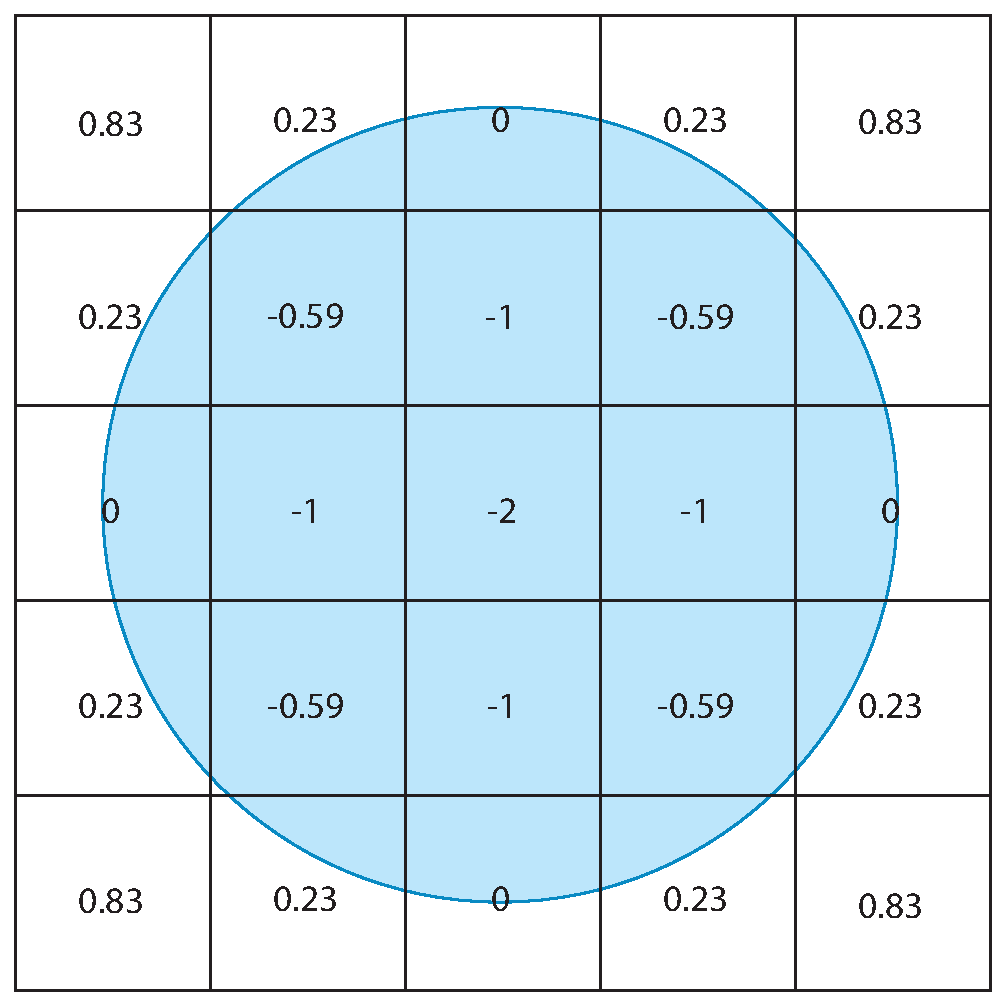
\includegraphics[width=90mm]{img/levelset.pdf}
\caption{A numerical example of a level set representing a sphere (blue).}
\label{levetsetexample}
\end{figure}

Another important feature of a level set is the gradient.

\begin{equation}
\nabla \phi = \hat{n}
\end{equation}

where $\hat{n}$ is the unit vector describing the direction to the closest point of the surface. This means, given spatial coordinates $\vec{x}$, one can easily find the closest point $\vec{x}_s$ on the surface. If we evaluate the level set at $\vec{x}$, i.e. $\phi(\vec{x})$, we get the distance to the surface. If we walk this distance in the negative direction of the gradient, we end up at the surface.

\begin{equation}
\vec{x}_s = \vec{x} - \phi(\vec{x})\nabla \phi(\vec{x})
\end{equation}
\noindent
For any level set operator, it is important that the length of the gradient is always of unit length. This is called the Eikonal equation.

\begin{equation}
|\nabla \phi| = 1
\label{eikonaleqfirst}
\end{equation}
